\documentclass[8pt]{beamer}


\mode<presentation>
{
\usetheme{Singapore} %use default if problems or Szeged
  % or ... https://deic-web.uab.cat/~iblanes/beamer_gallery/index_by_theme.html
}
\setbeamertemplate{footline}[frame number]
\usepackage{booktabs}
\usepackage{color}

\usepackage[english]{babel}
% or whatever

\usepackage[latin1]{inputenc}
% or whatever

\usepackage{times}
\usepackage[T1]{fontenc}
% Or whatever. Note that the encoding and the font should match. If T1
% does not look nice, try deleting the line with the fontenc.
\usepackage[super]{nth}
\usepackage{xcolor}
\usepackage{relsize} %large math 

\usepackage{graphicx} % to insert the logo

\usepackage[font=scriptsize,skip=1pt]{caption}

\setbeamertemplate{caption}[numbered]

\title[S.I.s.a.R. Model] % (optional, use only with long paper titles)
{An Agent-Based Model of the Covid-19 epidemic, using Genetic Algorithms to optimize vaccinations: a very short presentation}

\author[] % (optional, use only with lots of authors)
{G.~Pescarmona\inst{1} \and P.~Terna\inst{2} \and A.~Acquadro\inst{1} \and P.~Pescarmona\inst{3} \and G.~Russo\inst{4}  
\and S.~Terna\inst{5}  }
% - Give the names in the same order as the appear in the paper.
% - Use the \inst{?} command only if the authors have different
%   affiliation.


\institute[] % (optional, but mostly needed)
{
  \inst{1}%
 University of Torino, Italy
  \and
  \inst{2}%
  University of Torino, Italy, retired \& Fondazione Collegio Carlo Alberto, Honorary Fellow, Italy
 \and
  \inst{3}%
  University of Groningen, The Netherlands  
  \and
  \inst{4}%
  Centro Einaudi, Torino, Italy
  \and
  \inst{5}%
 tomorrowdata.io
  }
% - Use the \inst command only if there are several affiliations.
% - Keep it simple, no one is interested in your street address.


\date[] % (optional, should be abbreviation of conference name)
{JPCS Mini-Conference -- April \nth{10}, 2021}

\begin{document}

%%%%%%%%%%%%%%%%%%%%%%%%%%%%%%%%%%%%%%%%%%%%%%%%%%%%%%%%%
\begin{frame}


\includegraphics[width=0.18\textwidth]{logo_unito.png}~~~
\includegraphics[width=0.15\textwidth]{CCA_Logo.png}

  \titlepage
\end{frame}

%%%%%%%%%%%%%%%%%%%%%%%%%%%%%%%%%%%%%%%%%%%%%%%%%%%%%%%%%
\section{Introduction}
%%%%%%%%%%%%%%%%%%%%%%%%%%%%%%%%%%%%%%%%%%%%%%%%%%%%%%%%%
\begin{frame}{Tool and links}

  \begin{itemize}

\item We use NetLogo, at \url{https://ccl.northwestern.edu/netlogo/}.

 \medskip
 
 \item
 
S.I.s.a.R. is at \url{https://terna.to.it/simul/SIsaR.html} with information on model construction, the draft of a preliminary paper also reporting results, and an online executable version of the simulation program, built using NetLogo.

 \medskip
 
 \item
 A short paper is published at \url{https://rofasss.org/2020/10/20/sisar/}
 
 \medskip
 
 G. Pescarmona, P. Terna, A. Acquadro, P. Pescarmona, G. Russo, and S. Terna. How Can ABM Models Become Part of the Policy-Making Process in Times of Emergencies---The SISAR Epidemic Model. \emph{RofASSS}, 2020.

 \end{itemize}
\end{frame}

%%%%%%%%%%%%%%%%%%%%%%%%%%%%%%%%%%%%%%%%%%%%%%%%%%%%%%%%%
\begin{frame}{The scale and the items (in Piedmont, a North-West Italian region with 4,350,000 residents)}

\begin{itemize}

\item $1:1000$.

\bigskip

\item Houses.
\item Schools.
\item Hospitals.
\item Nursing homes,
\item Factories.

\end{itemize}

\end{frame}
%%%%%%%%%%%%%%%%%%%%%%%%%%%%%%%%%%%%%%%%%%%%%%%%%%%%%%%%%
\section{The model}


%%%%%%%%%%%%%%%%%%%%%%%%%%%%%%%%%%%%%%%%%%%%%%%%%%%%%%%%%
\begin{frame}{The world 3D}

\begin{figure}[H]
\center
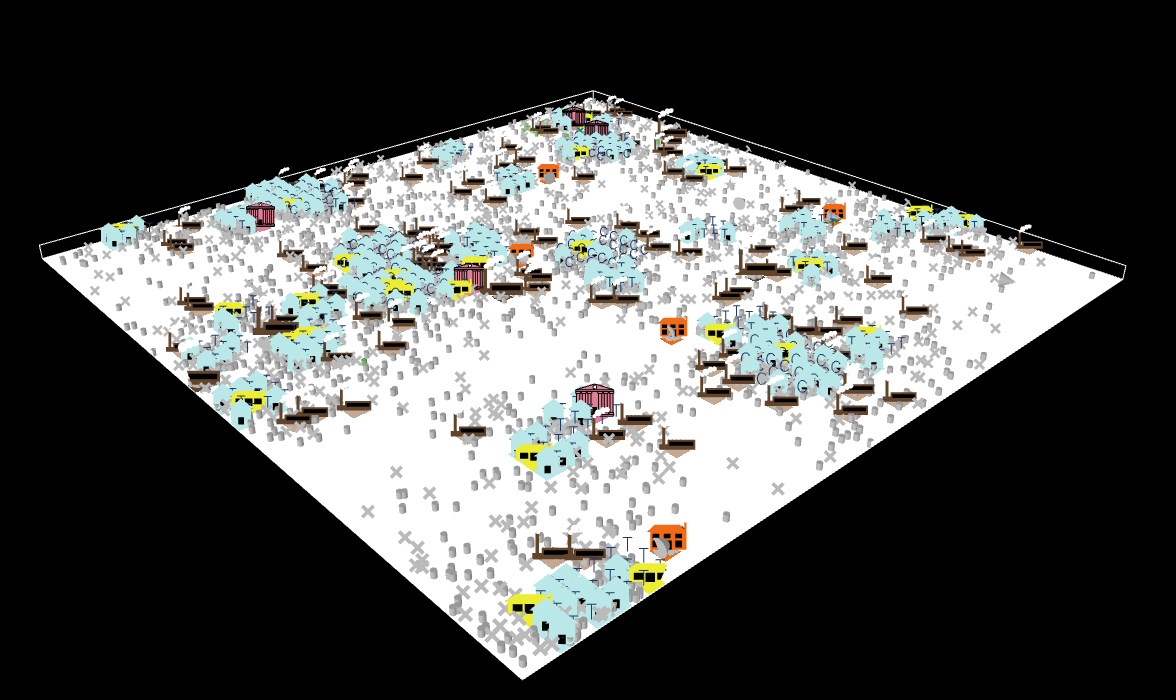
\includegraphics[scale=0.55]{world3D.png}

\caption{The world 3D} 
\label{world3D}
\end{figure}

\end{frame}

%%%%%%%%%%%%%%%%%%%%%%%%%%%%%%%%%%%%%%%%%%%%%%%%%%%%%%%%%
\section{Exploring cases}

%%%%%%%%%%%%%%%%%%%%%%%%%%%%%%%%%%%%%%%%%%%%%%%%%%%%%%%%%
\subsection{Simulation batches}

%%%%%%%%%%%%%%%%%%%%%%%%%%%%%%%%%%%%%%%%%%%%%%%%%%%%%%%%%
\begin{frame}{Simulation batches}

  \begin{itemize}
  \item

We explore systematically the introduction of factual, counterfactual, and prospective interventions to control the spread of the contagions. 

  \item
Each simulation run---whose length corresponds to the disappearance of symptomatic or asymptomatic contagion cases---is a datum in a wide scenario of variability in time and effects.   
  
  \item
We need to represent compactly the results  emerging from batches of simulation repetitions, to compare the  consequences of the basic assumptions adopted for each specific batch.

 \item
Besides summarizing the results with the usual statistical indicators, we adopt the technique of the heat-maps.

\item
Each heat-map reports the duration of each simulated epidemic in the $x$ axis and the number of the symptomatic, asymptomatic, and deceased agents in the $y$ axis. The $z$ axis is represented by the colors, as in the logarithmic scale on the right of each picture. 

\item
In our batches we have 10,000 runs.

\end{itemize}
\end{frame}

%%%%%%%%%%%%%%%%%%%%%%%%%%%%%%%%%%%%%%%%%%%%%%%%%%%%%%%%%
\subsection{Epidemics without and with control}

%%%%%%%%%%%%%%%%%%%%%%%%%%%%%%%%%%%%%%%%%%%%%%%%%%%%%%%%%
\begin{frame}{10,000 epidemics without control in Piedmont}

% readRunResults10kStableSeedsCPoints_noControl_ChangingWorld_plusHMlog

\begin{table}[H]
\center
\tiny

\begin{tabular}{lrrr}
\toprule
{} &  symptomatic &  totalInfected\&Deceased &  duration \\
\midrule
count &     10000.00 &                10000.00 &  10000.00 \\
mean  &       969.46 &                 2500.45 &    303.10 \\
std   &       308.80 &                  802.88 &     93.50 \\
\bottomrule
\end{tabular}

\label{noCTab}
%\caption{a caption}
\end{table}

\begin{figure}[H]
\center
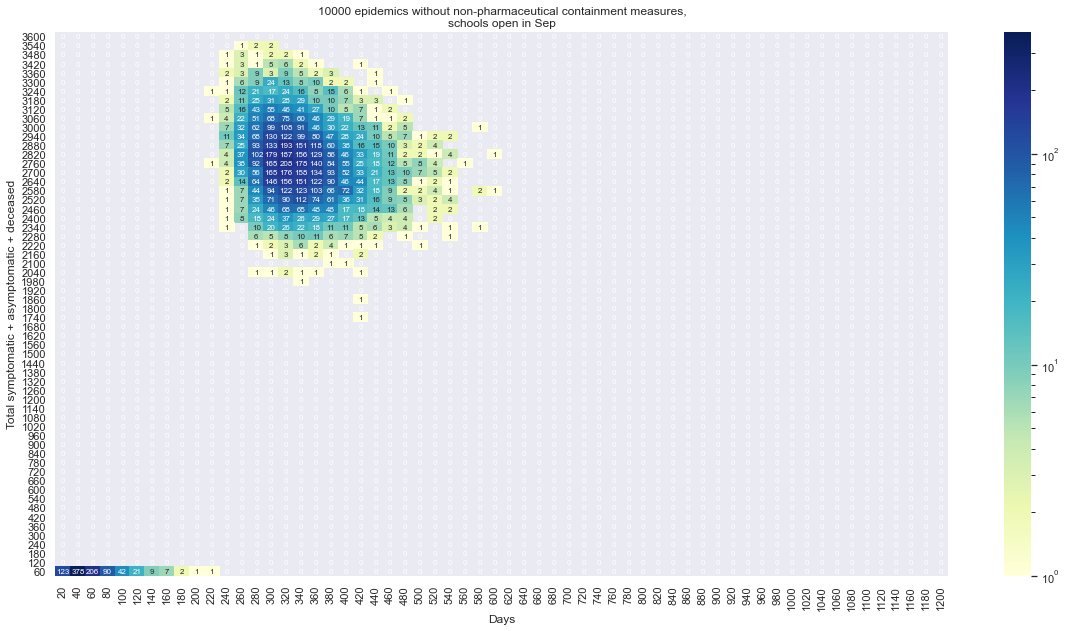
\includegraphics[scale=0.22]{10kNoControl.png}
\caption{Without non-pharmaceutical containment measures} 
\label{noC}
\end{figure}

\end{frame}


%%%%%%%%%%%%%%%%%%%%%%%%%%%%%%%%%%%%%%%%%%%%%%%%%%%%%%%%%
\begin{frame}{10,000 epidemic with basic control in Piedmont, first wave}

% readRunResults10kStableSeedsCPoints_basicControlB_schoolOpenSeptChangingWorld_plusHMlog

\begin{table}[H]
\center
\tiny

\begin{tabular}{lrrr}
\toprule
{} &  symptomatic &  totalInfected\&Deceased &  duration \\
\midrule
count &     10000.00 &                10000.00 &  10000.00 \\
mean  &       344.22 &                  851.64 &    277.93 \\
std   &       368.49 &                  916.41 &    213.48 \\
\bottomrule
\end{tabular}

\label{basicCTab}
%\caption{a caption}
\end{table}

\begin{figure}[H]
\center
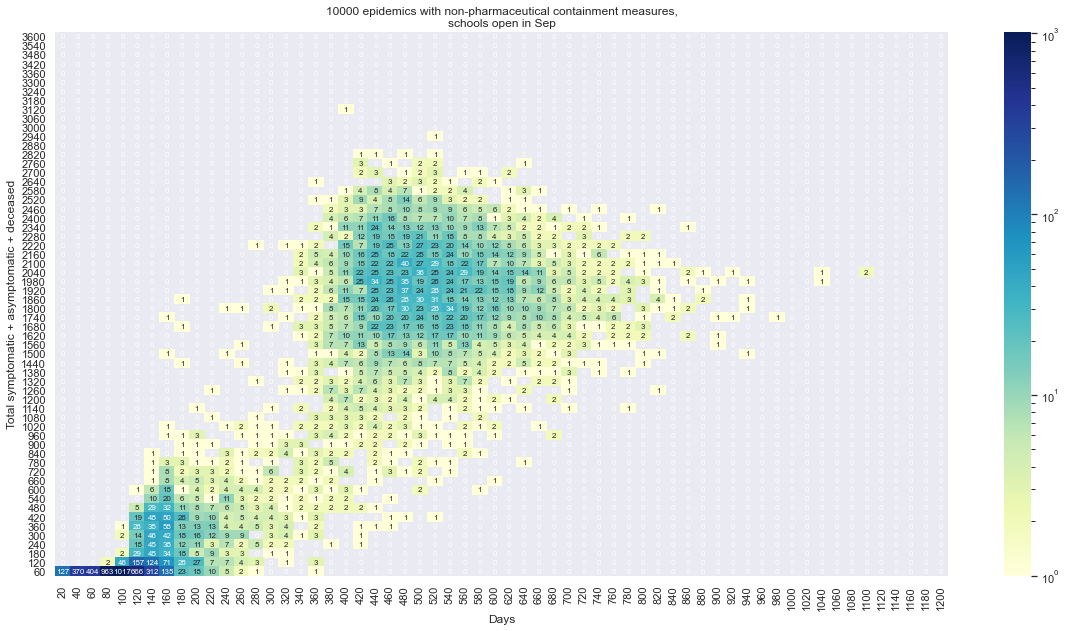
\includegraphics[scale=0.22]{10kBasicC.png}
\caption{First wave with non-pharmaceutical containment measures} 
\label{basicC}
\end{figure}

\end{frame}



%3%%%%%%%%%%%%%%%%%%%%%%%%%%%%%%%%%%%%%%%%%%%%%%%%%%%%%%%%
\begin{frame}{Second w., new infections from outside, with new specific measures}

% selectResults10kStableSeedsCPoints_basicControlB_schoolOpenSeptOctMarControlChangingWorldNewStart_plusHMlog.ipynb
% using 10kCtrl1NStartCtrl2M.csv from SIsaR_0.9.5.4.1trials10kCtrl1NStartCtrl2M.nlogo

\textbf{1407} {\tiny epidemics stable in Summer 2020 out of 10,000, rule: at Jun~1,~20 select if sym. (10, 70], actual v. 33.3 \& at Sep~20,~20 select if sym. (20, 90], actual value 37.5;} \textbf{874} {\tiny at Dec~15,~20, rule: sym.+asym.>Sep~20,~20, actual value: 200.0.}

\begin{figure}[H]
\center
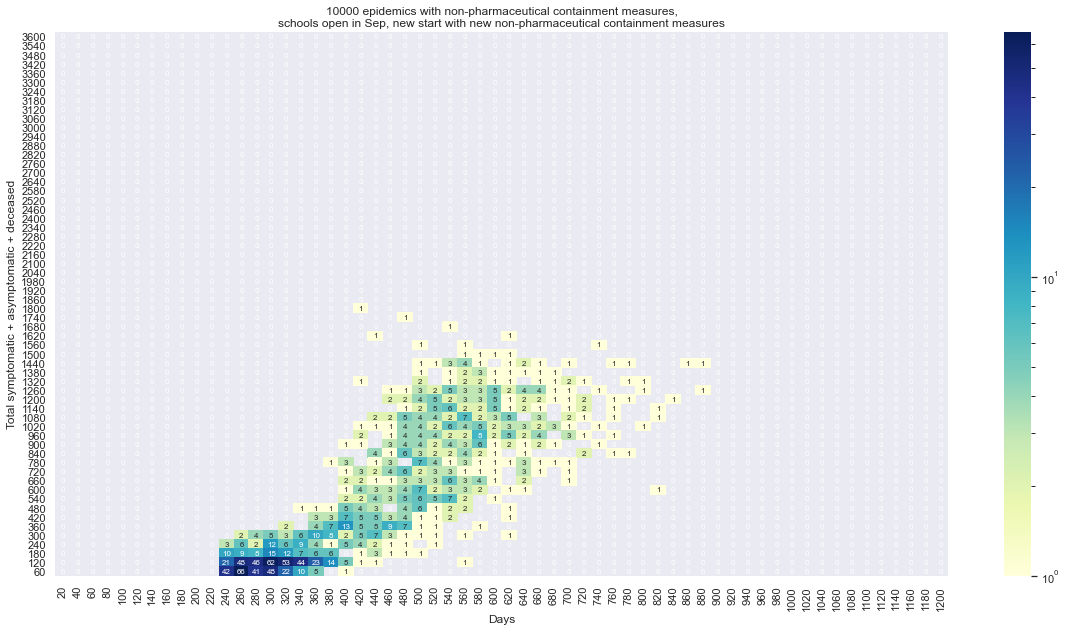
\includegraphics[scale=0.17]{10kForceWave2Contr2.png}
\caption{First wave with non-ph.containment measures, forcing the second wave, \textbf{with new specific non-ph. containment measures}}
\label{selForceWave2Contr2}
\end{figure}

%\vspace{-0.4cm}

\begin{table}[H]
\center
\tiny
\begin{tabular}{p{0.4cm}p{0.3cm}p{0.3cm}p{0.3cm}p{0.3cm}p{0.3cm}p{0.3cm}p{0.3cm}p{0.3cm}p{0.3cm}p{0.3cm}p{0.3cm}p{0.3cm}p{0.4cm}}
\toprule
(1000) &  Jun~1,~20 & &  Sep~9,~20 & & Dec~15,~20 & & Feb~1,~21 & & May~1,~21 & & Dec~15,~20~~~to~~~end   \\
cum.~v. &  sym. &  all &  sympt. &  totalInf. &  sympt. &  totalInf. &  sympt. &  totalInf. &  sympt. &  totalInf. &  sympt. &  totalInf.  & days\\
\midrule
count &   1407.0 &                     1407.0 &   1407.0 &                     1407.0 &    874.0 &                      874.0 &    719.0 &                      719.0 &    523.0 &                      523.0 &              874.0 &                   874.0 &  874.0 \\
mean  &     35.6 &                       72.7 &     40.0 &                       84.1 &    \textbf{130.0} &                      \textbf{340}.6 &    \textbf{194.4} &                      \textbf{512.8} &    \textbf{295.7} &                      \textbf{791.2} &               252.7 &                   666.4 &  494.1 \\
std   &     14.1 &                       42.6 &     16.7 &                       52.8 &     83.9 &                      232.6 &    104.1 &                      276.9 &    119.1 &                      300.6 &               156.8 &                   416.4 &  122.7 \\
\bottomrule
\end{tabular}

\label{selSpontWave2Contr2Tab}
%\caption{a caption}
\end{table}


\end{frame}

%%%%%%%%%%%%%%%%%%%%%%%%%%%%%%%%%%%%%%%%%%%%%%%%%%%%%%%%%
\begin{frame}{Fragile persons and future considerations}

\begin{itemize}

\item A quite impressive analysis  in Nature, Feb. 16, 2021, 
\emph{The coronavirus is here to stay---here's what that means}

\medskip

\url{https://www.nature.com/articles/d41586-021-00396-2}

\medskip

\emph{A Nature survey shows many scientists expect the virus that causes COVID-19 to become endemic, but it could pose less danger over time}.

\medskip

\item
If Nature is right, a possible long-term strategy is to stop all fragile people for a given period when $R_t$ starts increasing (also with fragile workers in sick leave, if unable to work remotely).

\medskip

With social benefits, e.g., schooling, and economic benefits, if activities do not stop

\medskip

\item Besides, mainly for the fragile people, adopt prevention and vaccinations.

\medskip

\item A note: the same strategy would also have been surprisingly efficient now, for the second wave.

\end{itemize}

\end{frame}



%5%%%%%%%%%%%%%%%%%%%%%%%%%%%%%%%%%%%%%%%%%%%%%%%%%%%%%%%%
\begin{frame}{Sec. w., new infect. from outs., stop fragile people. 60  days from Oct. 5\footnote{Schools are always working 100\% in this case.}}

%selectResults10kStableSeedsCPoints_basicControlB_schoolOpenSeptNoFragOCT05-60dControlChangingWorldNewStart_plusHMlog.ipynb
% using 10kCtrl1NStartNoFragOCT05-60d.csv from SIsaR_0.9.5.4.1trials10kCtrl1NStartNoFragOCT05-60d.nlogo

\textbf{1407} {\tiny epidemics stable in Summer 2020 out of 10,000, rule: at Jun~1,~20 select if sym. (10, 70], actual v. 33.3 \& at Sep~20,~20 select if sym. (20, 90], actual value 37.5;} \textbf{886} {\tiny at Dec~15,~20, rule: sym.+asym.>Sep~20,~20, actual value: 200.0.}

\begin{figure}[H]
\center
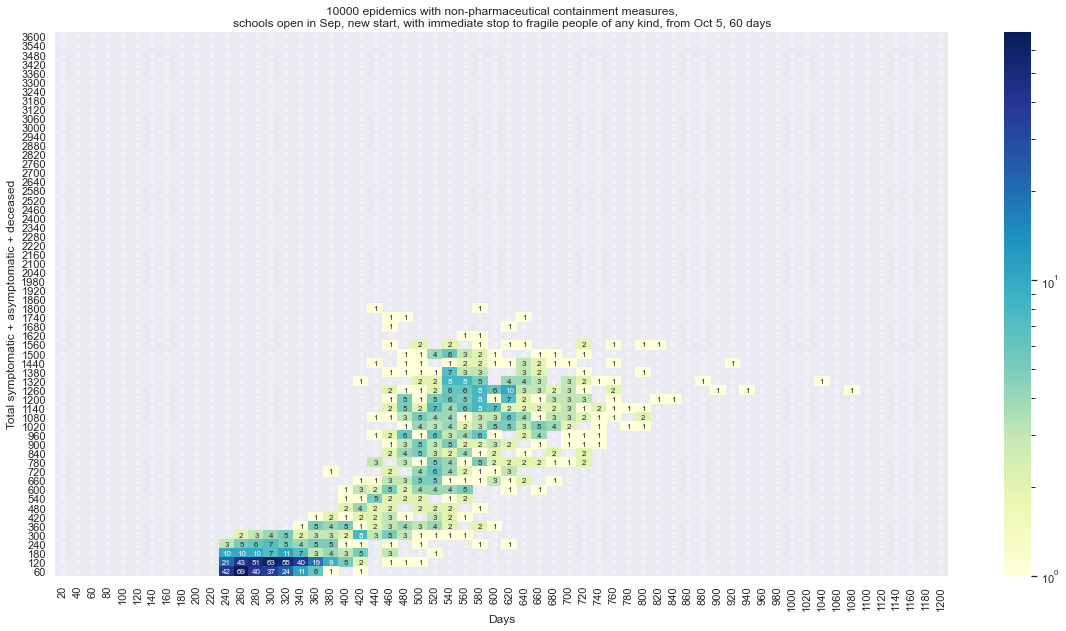
\includegraphics[scale=0.17]{10kForceWave2NoFragOct5for60d.png}
\caption{First wave with non-ph, cont, meas., forcing the sec. w.; \textbf{in sec. w., uniquely stop fragile people, including fragile workers}} 
\label{selForceWave2NoFrag}
\end{figure}

%\vspace{-0.4cm} 

\begin{table}[H]
\center
\tiny
\begin{tabular}{p{0.3cm}p{0.3cm}p{0.3cm}p{0.3cm}p{0.3cm}p{0.3cm}p{0.3cm}p{0.3cm}p{0.3cm}p{0.3cm}p{0.3cm}p{0.3cm}p{0.3cm}p{0.4cm}}
\toprule
(1000) &  Jun~1,~20 & &  Sep~9,~20 & & Dec~15,~20 & & Feb~1,~21 & & May~1,~21 & & Dec~15,~20~~~to~~~end   \\
{} &  sym. &  all &  sympt. &  totalInf. &  sympt. &  totalInf. &  sympt. &  totalInf. &  sympt. &  totalInf. &  sympt. &  totalInf.  & days\\
\midrule
count &   1407.0 &                     1407.0 &   1407.0 &                     1407.0 &    886.0 &                      886.0 &    761.0 &                      761.0 &    637.0 &                      637.0 &              886.0 &                   886.0 &  886.0 \\
mean  &     35.6 &                       72.7 &     40.0 &                       84.1 &    \textbf{{\color{cyan}128.1}} &                      \textbf{{\color{cyan}326.3}} &    \textbf{211.0} &                      \textbf{555.1} &    \textbf{323.3} &                      \textbf{862.1} &               301.1 &                   792.3 &  515.5 \\
std   &     14.1 &                       42.6 &     16.7 &                       52.8 &     89.6 &                      234.2 &    118.1 &                      306.7 &    126.4 &                      315.9 &               170.7 &                   450.2 &  116.9 \\
\bottomrule
\end{tabular}

\label{selForceWave2NoFragTab}
%\caption{a caption}
\end{table}


\end{frame}





%%%%%%%%%%%%%%%%%%%%%%%%%%%%%%%%%%%%%%%%%%%%%%%%%%%%%%%%%
\section{Planning vaccination campaigns}

%%%%%%%%%%%%%%%%%%%%%%%%%%%%%%%%%%%%%%%%%%%%%%%%%%%%%%%%%
\begin{frame}{Planning a vaccination campaign}

\begin{itemize}
\item Exploring vaccination sequences, using \emph{genetic algorithms}. A detailed note, frequently updated, is at \url{https://terna.to.it/simul/GAresultPresentation.pdf}.

\bigskip

\item We compare the effect of choosing vaccination quotas via GAs with two predetermined strategies.

\bigskip

\item Key dates: 
\begin{itemize}
\item in the internal calendar of the model, day 373 is Feb. \nth{12}, 2021, which is effectively the starting point of the vaccinations in the region; 

\item the day of the effectiveness of the initial vaccinations, 40 days later, is day 413 (Mar. \nth{22}, 2021).
\end{itemize}

\end{itemize}

\end{frame}

%%%%%%%%%%%%%%%%%%%%%%%%%%%%%%%%%%%%%%%%%%%%%%%%%%%%%%%%%
\begin{frame}{Vaccination groups}

We take into consideration seven groups in order of decreasing fragility but also considering the exposure to contagion:

\begin{enumerate}
\item [\emph{g1}]
	extra fragile people with three components;
	\begin{itemize}
		\item due to intrinsic characteristics: people in nursing homes;
		\item due to risk exposure:
		\begin{itemize}
			\item nursing homes operators;
			\item healthcare operators;
 		\end{itemize} 
 	\end{itemize}  
\item [\emph{g2}]
	teachers;
\item [\emph{g3}]
	workers with medical fragility;
\item [\emph{g4}]
	regular workers;
\item [\emph{g5}]
	fragile people without special characteristics;
\item [\emph{g6}]
	regular people, not young, not worker, and not teacher;
\item [\emph{g7}]
	young people excluding special activity cases (a limited number in \emph{g1}).
\end{enumerate}

\end{frame}

%%%%%%%%%%%%%%%%%%%%%%%%%%%%%%%%%%%%%%%%%%%%%%%%%%%%%%%%%
\begin{frame}{Vaccination sequence, \emph{wise} strategy}

\begin{figure}[H]
\center
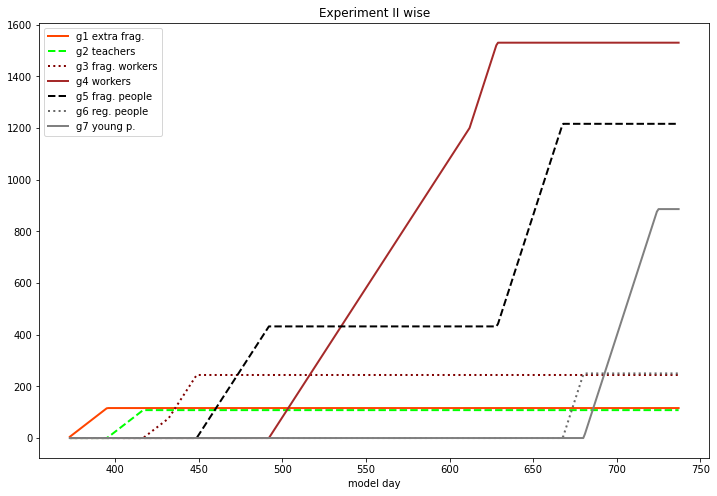
\includegraphics[scale=0.4]{Experiment_II_wiseVaccinationSequence.png} % experiment_II_vaccination_plots.ipynb

\caption{A ``wise'' vaccination sequence} 
\label{Experiment_II_wiseVaccinationSequence}
\end{figure}




\end{frame}

%%%%%%%%%%%%%%%%%%%%%%%%%%%%%%%%%%%%%%%%%%%%%%%%%%%%%%%%%
\begin{frame}{GAs vaccination sequence, with vaccinated people still spreading the infection}


\begin{figure}[H]
\center
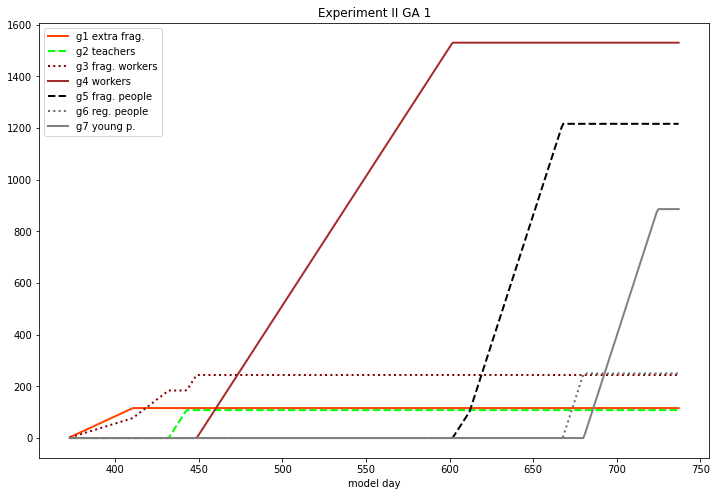
\includegraphics[scale=0.4]{Experiment_II_GA_1_VaccinationSequence.png} % experiment_II_vaccination_plots.ipynb

\caption{GAs vaccination sequence} 
\label{Experiment_II_GA1VaccinationSequence}
\end{figure}



\end{frame}

%%%%%%%%%%%%%%%%%%%%%%%%%%%%%%%%%%%%%%%%%%%%%%%%%%%%%%%%%
\begin{frame}{Synopsys}

Three hypotheses about contagion transmission from vaccinated people, if infected: 100\%, never, 50\%.

\medskip

\begin{table}[H]
\centering
\begin{scriptsize} % or footnotesize, scriptsize, tiny, etc.
\begin{tabular}{llllllllllll}
\toprule
Case    & At   & Final      & Final        & Final       & Final      & Final       & Final    & Final        & Final    & Final        & Final     \\
             & day & no         & plain       & wise        & GAs         & plain       & wise        & GAs         & plain       & wise        & GAs    \\
             & 413 & vaccin. & vaccin.    & vaccin.  & vaccin.  & vaccin.  & vaccin.  & vaccin.  & vaccin.  & vaccin.  & vaccin.  \\
 (1000) &        &              &  infect.  &  infect. &  infect. &  infect. &  infect. &  infect. &  infect. &  infect. &  infect.\\
             &       &              &  100\%   &  100\% &  100\% &  0\% &  0\% &  0\% & 50\% &  50\% &  50\% \\
\midrule
I            & 197 & 325 & 236 & 263 & \textbf{200} & 203 & 211   & 199 & 204 & 229 & 203 \\
             & -      & 128 & 39    & 66  & \textbf{3}    &  6     & 14  & 2     & 7     & 32 & 6 \\
\\
II           & 233 & 375 & 355 &  344 & \textbf{305}  & 340 & 334 & \textbf{297}  & 356 & 344 &  \textbf{288} \\
             & -      &  142 & 122 & 111 & \textbf{72}    & 107 & 101 & \textbf{64}   & 123   & 111 &  \textbf{55} \\
\\
\bottomrule  
\end{tabular}
\end{scriptsize}
\caption{Results of the campaigns in the two cases, only symptomatic people (second row in each case: minus day 413)}
\label{caseSynopsys}
\end{table}

\end{frame}

%%%%%%%%%%%%%%%%%%%%%%%%%%%%%%%%%%%%%%%%%%%%%%%%%%%%%%%%%
\section{My home}

%%%%%%%%%%%%%%%%%%%%%%%%%%%%%%%%%%%%%%%%%%%%%%%%%%%%%%%%%
\begin{frame}

\center
\begin{large}
\url{https://terna.to.it}
\end{large}

\end{frame}

\end{document}